% Gabarit pandoc des corrigés publiés (brut et guidé). Contenu sans marque ni nom de site.
% Compilation : lualatex (latexmk -lualatex).
% Le Markdown reste la source unique : ne pas éditer ce fichier .tex à la main.
\documentclass[11pt,a4paper]{article}

% --- Moteur, polices (Latin Modern) et langue ---------------------------------
\usepackage{iftex}
\ifLuaTeX\else\errmessage{Ce document se compile avec lualatex}\fi
\usepackage{amsmath,amssymb,mathtools}
\usepackage{fontspec}
% mathrm=sym : \mathrm prend ses glyphes dans la police mathématique (ℓ, μ, Ω), comme KaTeX.
\usepackage[math-style=TeX,bold-style=TeX,mathrm=sym]{unicode-math}
% Repli pour les glyphes absents de Latin Modern (indices et exposants Unicode,
% flèches, filets des schémas en texte, symboles) : DejaVu, puis Latin Modern Math
% (ℓ, lettres mathématiques Unicode des légendes).
\directlua{
  luaotfload.add_fallback("repliTexte", {"DejaVuSerif:mode=harf;", "DejaVuSans:mode=harf;", "file:latinmodern-math.otf:mode=harf;"})
  luaotfload.add_fallback("repliMono", {"DejaVuSansMono:mode=harf;", "DejaVuSans:mode=harf;", "file:latinmodern-math.otf:mode=harf;"})
}
\setmainfont{Latin Modern Roman}[RawFeature={fallback=repliTexte}]
\setsansfont{Latin Modern Sans}[RawFeature={fallback=repliTexte}]
\setmonofont{Latin Modern Mono}[RawFeature={fallback=repliMono}]
\setmathfont{Latin Modern Math}
\usepackage[french]{babel}
\frenchsetup{SmallCapsFigTabCaptions=false}

% --- Mise en page --------------------------------------------------------------
\usepackage[a4paper,margin=2.2cm,headheight=14pt,footskip=1.2cm]{geometry}
\usepackage{microtype}
\setlength{\emergencystretch}{4em}
\tolerance=1500
\setlength{\parindent}{0pt}
\setlength{\parskip}{0.55\baselineskip plus 2pt minus 1pt}
\usepackage{xcolor}
% Gris nommés : babel-french rend « ! » actif dans le document.
\definecolor{gris2}{gray}{0.98}
\definecolor{gris3}{gray}{0.97}
\definecolor{gris5}{gray}{0.95}
\definecolor{gris35}{gray}{0.65}
\definecolor{gris40}{gray}{0.60}
\definecolor{gris45}{gray}{0.55}
\definecolor{gris50}{gray}{0.50}
\definecolor{gris55}{gray}{0.45}
\definecolor{gris60}{gray}{0.40}
\definecolor{gris65}{gray}{0.35}
\definecolor{gris70}{gray}{0.30}
\definecolor{gris80}{gray}{0.20}
\definecolor{gris85}{gray}{0.15}
\usepackage{graphicx}
\usepackage{float}
\usepackage{caption}
\captionsetup{font=small,labelformat=empty,justification=centering}
\usepackage{booktabs,longtable,array,multirow,calc}
\usepackage{siunitx}
\sisetup{locale=FR}
\usepackage[version=4]{mhchem}
\usepackage{listings}
\usepackage{fancyhdr}
\usepackage{lastpage}
\usepackage[most]{tcolorbox}
\usepackage{enumitem}
\setlist{nosep,leftmargin=*,topsep=2pt}
\usepackage[hidelinks,unicode]{hyperref}
\usepackage{bookmark}
\hypersetup{pdftitle={CCINP TSI — Mathématiques 2026},pdfauthor={Rédigé par IA},pdfcreator={LaTeX},pdfsubject={Corrigé brut}}
\usepackage{xurl}

% --- Pandoc : listes, tableaux, figures ----------------------------------------
\providecommand{\passthrough}[1]{#1}
\providecommand{\tightlist}{\setlength{\itemsep}{0pt}\setlength{\parskip}{0pt}}

\makeatletter
\def\maxwidth{\ifdim\Gin@nat@width>\linewidth\linewidth\else\Gin@nat@width\fi}
\def\maxheight{\ifdim\Gin@nat@height>0.55\textheight 0.55\textheight\else\Gin@nat@height\fi}
\makeatother
\setkeys{Gin}{width=\maxwidth,height=\maxheight,keepaspectratio}
\setcounter{secnumdepth}{-\maxdimen}
\providecommand{\pandocbounded}[1]{#1}

% --- Code (listings) -----------------------------------------------------------
\lstset{
  basicstyle=\ttfamily\small,
  columns=fullflexible,
  keepspaces=true,
  breaklines=true,
  breakatwhitespace=false,
  postbreak=\mbox{\textcolor{gris50}{$\hookrightarrow$}\space},
  frame=single,
  rulecolor=\color{gris35},
  framesep=4pt,
  xleftmargin=5pt,xrightmargin=5pt,
  backgroundcolor=\color{gris3},
  keywordstyle=\bfseries,
  commentstyle=\color{gris65},
  stringstyle=\color{gris80},
  showstringspaces=false,
  tabsize=4,
  extendedchars=true,
  aboveskip=6pt,belowskip=6pt,
}

% --- Macros des corrigés (KaTeX ↔ LaTeX) ---------------------------------------
% Les corrigés sont écrits pour KaTeX : on définit ici ce que KaTeX connaît et
% que LaTeX n'a pas, sans jamais retoucher le Markdown.
\providecommand{\R}{\mathbb{R}}
\providecommand{\N}{\mathbb{N}}
\providecommand{\Z}{\mathbb{Z}}
\providecommand{\Q}{\mathbb{Q}}
\providecommand{\C}{\mathbb{C}}
\providecommand{\dd}{\mathrm{d}}
\providecommand{\llbracket}{\lBrack}
\providecommand{\rrbracket}{\rBrack}
\providecommand{\lBrace}{\lbrace}
\providecommand{\rBrace}{\rbrace}
\providecommand{\Box}{\square}
\providecommand{\Diamond}{\lozenge}
\providecommand{\varnothing}{\emptyset}
\providecommand{\argmax}{\operatorname*{arg\,max}}
\providecommand{\argmin}{\operatorname*{arg\,min}}
\renewcommand{\leq}{\leqslant}
\renewcommand{\geq}{\geqslant}

% Équation hors texte : réduite à la largeur de la ligne si elle déborde.
\newsavebox{\boiteequation}
\newcommand{\equationajustee}[1]{%
  \sbox{\boiteequation}{$\displaystyle #1$}%
  \ifdim\wd\boiteequation>\linewidth
    \[\resizebox{\linewidth}{!}{\usebox{\boiteequation}}\]%
  \else
    \[#1\]%
  \fi}

% --- Encadrés pédagogiques (sobres, lisibles en noir et blanc) -----------------
\tcbset{
  encadre/.style={
    enhanced,breakable,sharp corners,
    colback=white,colframe=gris55,
    boxrule=0.4pt,leftrule=2.2pt,
    left=6pt,right=6pt,top=3pt,bottom=3pt,
    before skip=6pt,after skip=6pt,
    fonttitle=\bfseries\small,coltitle=black,
    attach title to upper,after title={\quad},
    parbox=false,
  }
}
\newtcolorbox{indication}[1]{encadre,colframe=gris45,colback=gris2,title={Indication~#1}}
\newtcolorbox{methode}{encadre,colframe=gris70,title={Méthode}}
\newtcolorbox{piege}{encadre,colframe=gris85,boxrule=0.8pt,leftrule=2.2pt,title={Piège}}
\newtcolorbox{jury}{encadre,colframe=gris60,colback=gris5,title={Jury}}
\newtcolorbox{encadrenote}{encadre,colframe=gris40}

% --- Titres de section ---------------------------------------------------------
\usepackage{titlesec}
\titleformat{\section}{\Large\bfseries}{}{0pt}{}
\titleformat{\subsection}{\large\bfseries}{}{0pt}{}
\titleformat{\subsubsection}{\normalsize\bfseries}{}{0pt}{}
\titlespacing*{\section}{0pt}{14pt plus 4pt minus 2pt}{6pt}
\titlespacing*{\subsection}{0pt}{10pt plus 3pt minus 2pt}{4pt}
\titlespacing*{\subsubsection}{0pt}{8pt plus 2pt minus 2pt}{2pt}

% --- En-tête et pied de page ---------------------------------------------------
\pagestyle{fancy}
\fancyhf{}
\fancyhead[L]{\small\textsc{Corrigé brut} · CCINP TSI}
\fancyhead[R]{\small Maths 2026}
\fancyfoot[L]{\footnotesize Corrigé rédigé par IA, non officiel}
\fancyfoot[R]{\footnotesize \thepage\,/\,\pageref*{LastPage}}
\renewcommand{\headrulewidth}{0.4pt}
\renewcommand{\footrulewidth}{0pt}
\fancypagestyle{plain}{\fancyhf{}\fancyfoot[R]{\footnotesize \thepage\,/\,\pageref*{LastPage}}\fancyfoot[L]{\footnotesize Corrigé rédigé par IA, non officiel}\renewcommand{\headrulewidth}{0pt}}

\begin{document}
\thispagestyle{plain}
\begin{center}
  {\small\scshape Corrigé brut}\par\smallskip
  {\LARGE\bfseries CCINP TSI — Mathématiques 2026\par}\medskip
  {\large CCINP · TSI · Maths · 2026\par}
\end{center}
\vspace{2pt}\hrule\vspace{8pt}

\emph{Corrigé rédigé par IA, non officiel. Signalez toute erreur.}

Épreuve de 4 heures, calculatrice interdite. Deux problèmes indépendants.

\begin{center}\rule{0.5\linewidth}{0.5pt}\end{center}

Problème 1 --- Calcul d'une intégrale via les nombres complexes

Dans tout le problème, \(a\) est un réel tel que \(|a|>1\).

\hypertarget{partie-i-lemme-pruxe9liminaire}{%
\section{Partie I --- Lemme préliminaire}\label{partie-i-lemme-pruxe9liminaire}}

\hypertarget{q1}{%
\subsection{Q1}\label{q1}}

Le trinôme réel \(P(z)=z^2-2az+1\) a pour discriminant

\equationajustee{\Delta=4a^2-4=4(a^2-1).}

Comme \(|a|>1\), on a \(a^2>1\), donc \(\Delta>0\). Le trinôme admet donc deux racines réelles distinctes, \(a-\sqrt{a^2-1}\) et \(a+\sqrt{a^2-1}\).

En les notant \(\alpha\) et \(\beta\), la factorisation d'un trinôme unitaire par ses racines donne :

\equationajustee{\boxed{\forall z\in\mathbb C,\quad z^2-2az+1=(z-\alpha)(z-\beta)}}

\equationajustee{\{\alpha,\beta\}=\big\{a-\sqrt{a^2-1},\ a+\sqrt{a^2-1}\big\}.}

En particulier \(\alpha\) et \(\beta\) sont \textbf{réels}.

\hypertarget{q2}{%
\subsection{Q2}\label{q2}}

Pour tout \(z\in\mathbb C\), on développe :

\equationajustee{(z-\alpha)(z-\beta)=z^2-(\alpha+\beta)z+\alpha\beta.}

Deux polynômes égaux en tout point ont les mêmes coefficients. Par identification avec \(z^2-2az+1\) :

\equationajustee{\boxed{\begin{aligned}\alpha+\beta&=2a\\ \alpha\beta&=1\end{aligned}}}

\hypertarget{q3}{%
\subsection{Q3}\label{q3}}

Par Q2, \(|\alpha|\,|\beta|=|\alpha\beta|=1\). Supposons \(|\alpha|\ge1\) et \(|\beta|\ge1\). Alors

\equationajustee{\begin{aligned}1=|\alpha|\,|\beta|&\ge|\alpha|\\ &\ge1,\end{aligned}}

donc \(|\alpha|=1\), puis \(|\beta|=1/|\alpha|=1\) :

\equationajustee{|\alpha|=|\beta|=1.}

Par Q2 et l'inégalité triangulaire dans \(\mathbb C\) :

\equationajustee{\begin{aligned}2|a|&=|\alpha+\beta|\\ &\le|\alpha|+|\beta|\\ &=2,\end{aligned}}

d'où

\equationajustee{\boxed{|a|\le1.}}

\hypertarget{q4}{%
\subsection{Q4}\label{q4}}

Q3 établit l'implication

\equationajustee{\big(|\alpha|\ge1\ \text{et}\ |\beta|\ge1\big)\Longrightarrow|a|\le1.}

Par contraposition, puisque \(|a|>1\), on n'a pas à la fois \(|\alpha|\ge1\) et \(|\beta|\ge1\) :

\equationajustee{\boxed{|\alpha|<1\quad\text{ou}\quad|\beta|<1.}}

Les deux ne peuvent avoir lieu simultanément, car \(|\alpha|\,|\beta|=1\). Avec la convention \(|\alpha|<1\) de l'énoncé : \(\alpha\) est réel et non nul (car \(\alpha\beta=1\)), donc \(\alpha\in\,]-1,1[\setminus\{0\}\).

De plus \(\beta=1/\alpha\), donc \(|\beta|>1\), et \(0<1-\alpha^2<1\).

\hypertarget{q5}{%
\subsection{Q5}\label{q5}}

Pour \(a=2\), le trinôme \(z^2-4z+1\) a pour discriminant \(\Delta=16-4=12>0\), et \(\sqrt{12}=2\sqrt3\). Ses racines sont

\equationajustee{\frac{4\pm2\sqrt3}2=2\pm\sqrt3.}

Comme \(1<\sqrt3<2\), on a \(0<2-\sqrt3<1<2+\sqrt3\). Avec \(|\alpha|<1\) :

\equationajustee{\boxed{\begin{aligned}\alpha&=2-\sqrt3\\ \beta&=2+\sqrt3\end{aligned}}}

Contrôle : \(\alpha+\beta=4=2a\) et \(\alpha\beta=4-3=1\).

\begin{figure}[H]
\centering
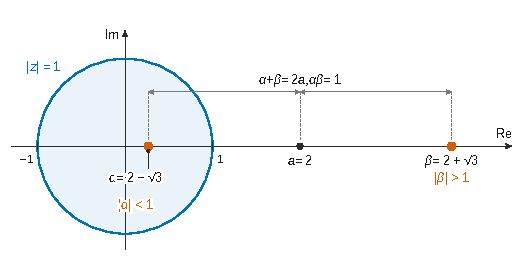
\includegraphics{figures/q5-racines-disque-unite.pdf}
\caption*{Figure 1 --- Racines de z² − 4z + 1 (a = 2) : α = 2 − √3 dans le disque
unité, β = 2 + √3 dehors, a milieu des deux}
\end{figure}

\hypertarget{partie-ii-calcul-dune-intuxe9grale}{%
\section{Partie II --- Calcul d'une intégrale}\label{partie-ii-calcul-dune-intuxe9grale}}

\hypertarget{ii.1-une-premiuxe8re-expression-en-suxe9rie-trigonomuxe9trique}{%
\subsection{II.1 --- Une première expression en série trigonométrique}\label{ii.1-une-premiuxe8re-expression-en-suxe9rie-trigonomuxe9trique}}

\hypertarget{q6}{%
\subsection{Q6}\label{q6}}

Soit \(t\in\mathbb R\). On a \(|\cos t|\le1\), donc, par l'inégalité triangulaire :

\equationajustee{\begin{aligned}|a-\cos t|&\ge|a|-|\cos t|\\ &\ge|a|-1\\ &>0.\end{aligned}}

D'où :

\equationajustee{\boxed{\forall t\in\mathbb R,\quad a-\cos t\ne0.}}

(Si \(a>1\), \(a-\cos t>0\) ; si \(a<-1\), \(a-\cos t<0\).)

\hypertarget{q7}{%
\subsection{Q7}\label{q7}}

\begin{itemize}
\tightlist
\item
  \emph{Continuité} : \(t\mapsto a-\cos t\) est continue sur \(\mathbb R\), comme différence d'une constante et de \(\cos\). Elle ne s'annule pas sur \(\mathbb R\) (Q6). Son inverse \(f\) est donc continue sur \(\mathbb R\).
\item
  \emph{Parité} : \(\mathbb R\) est symétrique par rapport à \(0\), et pour tout \(t\in\mathbb R\), \(f(-t)=\dfrac1{a-\cos(-t)}=f(t)\), car \(\cos\) est paire.
\item
  \emph{Périodicité} : pour tout \(t\in\mathbb R\), \(t+2\pi\in\mathbb R\) et \(f(t+2\pi)=f(t)\), car \(\cos\) est \(2\pi\)-périodique.
\end{itemize}

\textbf{\(f\) est continue, paire et \(2\pi\)-périodique sur \(\mathbb R\).}

\hypertarget{q8}{%
\subsection{Q8}\label{q8}}

\(f\) est \(2\pi\)-périodique et continue, donc continue par morceaux. Ses coefficients de Fourier trigonométriques sont :

\equationajustee{\boxed{\begin{aligned}a_0&=\frac1{2\pi}\int_0^{2\pi}f(t)\,\mathrm dt\\ a_n&=\frac1\pi\int_0^{2\pi}f(t)\cos(nt)\,\mathrm dt\quad(n\ge1)\\ b_n&=\frac1\pi\int_0^{2\pi}f(t)\sin(nt)\,\mathrm dt\quad(n\ge1)\end{aligned}}}

Le coefficient \(a_0\) est la valeur moyenne de \(f\) : c'est cette convention qui donne la forme \(\sum_{n\ge0}a_n\cos(nt)\) de Q9.

De plus, pour \(n\ge1\), \(t\mapsto f(t)\sin(nt)\) est impaire et \(2\pi\)-périodique. L'intégrale sur une période pouvant se prendre sur \([-\pi,\pi]\) :

\equationajustee{b_n=\frac1\pi\int_{-\pi}^{\pi}f(t)\sin(nt)\,\mathrm dt=0.}

\hypertarget{q9}{%
\subsection{Q9}\label{q9}}

La fonction \(t\mapsto a-\cos t\) est de classe \(\mathcal C^\infty\) et ne s'annule pas.

Donc \(f\) est de classe \(\mathcal C^\infty\) sur \(\mathbb R\), a fortiori \(\mathcal C^1\) par morceaux, et elle est \(2\pi\)-périodique.

Par le théorème de Dirichlet, la série de Fourier de \(f\) converge en tout point \(t\) vers \(\frac12\big(f(t^+)+f(t^-)\big)\), qui vaut \(f(t)\) puisque \(f\) est continue. Comme \(b_n=0\) (Q8) :

\equationajustee{\boxed{\begin{aligned}\forall t\in\mathbb R,\quad f(t)&=a_0+\sum_{n=1}^{+\infty}a_n\cos(nt)\\ &=\sum_{n=0}^{+\infty}a_n\cos(nt).\end{aligned}}}

\hypertarget{ii.2-une-seconde-expression-en-suxe9rie-trigonomuxe9trique}{%
\subsection{II.2 --- Une seconde expression en série trigonométrique}\label{ii.2-une-seconde-expression-en-suxe9rie-trigonomuxe9trique}}

\hypertarget{q10}{%
\subsection{Q10}\label{q10}}

Soit \(t\in\mathbb R\). Par la formule d'Euler \(\cos t=\frac{e^{it}+e^{-it}}2\) :

\equationajustee{\begin{aligned}2e^{it}(a-\cos t)&=2ae^{it}-e^{2it}-1\\ &=-\big((e^{it})^2-2ae^{it}+1\big).\end{aligned}}

Le membre de gauche est non nul (Q6 et \(e^{it}\ne0\)), donc le trinôme aussi. En divisant :

\equationajustee{\boxed{\forall t\in\mathbb R,\quad \frac1{a-\cos t}=\frac{-2e^{it}}{(e^{it})^2-2ae^{it}+1}.}}

\hypertarget{q11}{%
\subsection{Q11}\label{q11}}

Par Q1 appliquée en \(z=e^{it}\), on a \((e^{it})^2-2ae^{it}+1=(e^{it}-\alpha)(e^{it}-\beta)\), d'où, avec Q10 :

\equationajustee{\forall t\in\mathbb R,\quad \frac1{a-\cos t}=\frac{-2e^{it}}{(e^{it}-\alpha)(e^{it}-\beta)}.}

Comme \(\beta=1/\alpha\) (Q2), on factorise :

\equationajustee{\begin{aligned}e^{it}-\alpha&=e^{it}(1-\alpha e^{-it})\\ e^{it}-\beta&=-\frac{1-\alpha e^{it}}{\alpha}\end{aligned}}

Ces quantités sont non nulles, car \(|e^{it}|=1\) alors que \(|\alpha|<1<|\beta|\). Donc

\equationajustee{\frac1{a-\cos t}=\frac{2\alpha}{(1-\alpha e^{-it})(1-\alpha e^{it})}.}

Or, en réduisant au même dénominateur :

\equationajustee{\begin{aligned}\frac{\alpha e^{-it}}{1-\alpha e^{-it}}+\frac1{1-\alpha e^{it}}&=\frac{\alpha e^{-it}-\alpha^2+1-\alpha e^{-it}}{(1-\alpha e^{-it})(1-\alpha e^{it})}\\ &=\frac{1-\alpha^2}{(1-\alpha e^{-it})(1-\alpha e^{it})}.\end{aligned}}

Puisque \(1-\alpha^2\ne0\) :

\equationajustee{\boxed{\forall t\in\mathbb R,\quad \frac1{a-\cos t}=\frac{2\alpha}{1-\alpha^2}\left(\frac{\alpha e^{-it}}{1-\alpha e^{-it}}+\frac1{1-\alpha e^{it}}\right).}}

\hypertarget{q12}{%
\subsection{Q12}\label{q12}}

La série entière \(\sum z^n\) converge pour \(|z|<1\). Pour \(|z|\ge1\), son terme général ne tend pas vers \(0\) et elle diverge grossièrement. Ainsi :

\equationajustee{\boxed{R=1}}

\equationajustee{\boxed{\forall z\in\mathbb C,\ |z|<1\ :\ \sum_{n=0}^{+\infty}z^n=\frac1{1-z}.}}

\hypertarget{q13}{%
\subsection{Q13}\label{q13}}

Soit \(t\in\mathbb R\). On a \(|\alpha e^{-it}|=|\alpha|<1\) et \(|\alpha e^{it}|=|\alpha|<1\) : les deux raisons sont de module strictement inférieur à 1. Par Q12 :

\equationajustee{\begin{aligned}\frac{\alpha e^{-it}}{1-\alpha e^{-it}}&=\alpha e^{-it}\sum_{n=0}^{+\infty}\alpha^ne^{-int}\\ &=\sum_{n=0}^{+\infty}\alpha^{n+1}e^{-i(n+1)t}\\ \frac1{1-\alpha e^{it}}&=\sum_{n=0}^{+\infty}\alpha^ne^{int}\end{aligned}}

D'où la première égalité. Les deux séries convergeant, on peut les ajouter terme à terme, après réindexation (\(m=n+1\) dans la première) :

\equationajustee{\begin{aligned}{}&\sum_{m=1}^{+\infty}\alpha^me^{-imt}+1+\sum_{m=1}^{+\infty}\alpha^me^{imt}\\ &=1+\sum_{m=1}^{+\infty}\alpha^m\big(e^{imt}+e^{-imt}\big)\\ &=1+2\sum_{m=1}^{+\infty}\alpha^m\cos(mt).\end{aligned}}

\equationajustee{\boxed{\begin{aligned}\frac{\alpha e^{-it}}{1-\alpha e^{-it}}+\frac1{1-\alpha e^{it}}&=\sum_{n=0}^{+\infty}\alpha^{n+1}e^{-i(n+1)t}+\sum_{n=0}^{+\infty}\alpha^ne^{int}\\ &=1+2\sum_{n=1}^{+\infty}\alpha^n\cos(nt).\end{aligned}}}

\hypertarget{q14}{%
\subsection{Q14}\label{q14}}

Par Q11 et Q13, pour tout \(t\in\mathbb R\) :

\equationajustee{\begin{aligned}f(t)&=\frac{2\alpha}{1-\alpha^2}\Big(1+2\sum_{n=1}^{+\infty}\alpha^n\cos(nt)\Big)\\ &=\frac{2\alpha}{1-\alpha^2}+\sum_{n=1}^{+\infty}\frac{4\alpha^{n+1}}{1-\alpha^2}\cos(nt),\end{aligned}}

soit

\equationajustee{\boxed{\begin{aligned}{}&\forall t\in\mathbb R,\quad f(t)=\sum_{n=0}^{+\infty}\gamma_n\cos(nt)\\ &\gamma_0=\frac{2\alpha}{1-\alpha^2},\qquad \gamma_n=\frac{4\alpha^{n+1}}{1-\alpha^2}\ \ (n\ge1)\end{aligned}}}

\hypertarget{q15}{%
\subsection{Q15}\label{q15}}

Pour \(n\ge1\) :

\equationajustee{|\gamma_n|=\frac{4|\alpha|}{1-\alpha^2}\,|\alpha|^n.}

C'est une constante fois le terme général d'une série géométrique de raison \(|\alpha|\in[0,1[\), donc convergente. \textbf{Donc \(\sum\gamma_n\) converge absolument.}

\hypertarget{ii.3-conclusion}{%
\subsection{II.3 --- Conclusion}\label{ii.3-conclusion}}

\hypertarget{q16}{%
\subsection{Q16}\label{q16}}

Soit \(t\in\mathbb R\). Les séries \(\sum a_n\cos(nt)\) (Q9) et \(\sum\gamma_n\cos(nt)\) (Q14) convergent, toutes deux de somme \(f(t)\).

Pour tout \(N\), la somme partielle \(\sum_{n=0}^Nu_n\cos(nt)\) est la différence des sommes partielles de ces deux séries. Par linéarité de la limite :

\equationajustee{\boxed{\begin{aligned}\forall t\in\mathbb R,\quad \sum_{n=0}^{+\infty}u_n\cos(nt)&=f(t)-f(t)\\ &=0.\end{aligned}}}

\hypertarget{q17}{%
\subsection{Q17}\label{q17}}

\textbf{a)} Soit \(g\) de classe \(\mathcal C^1\) sur \(\mathbb R\) et \(T\)-périodique : \(g(t+T)=g(t)\) pour tout \(t\in\mathbb R\).

La fonction \(t\mapsto g(t+T)\) est la composée de \(g\) et de \(t\mapsto t+T\) ; elle est dérivable de dérivée \(t\mapsto g'(t+T)\). En dérivant les deux membres de l'égalité, qui sont deux fonctions égales sur \(\mathbb R\) :

\equationajustee{\forall t\in\mathbb R,\quad g'(t+T)=g'(t).}

\textbf{\(g'\) est \(T\)-périodique.}

\textbf{b)} La fonction \(t\mapsto a-\cos t\) est de classe \(\mathcal C^\infty\) sur \(\mathbb R\), et son dénominateur ne s'annule pas (Q6).

L'inverse d'une fonction de classe \(\mathcal C^\infty\) qui ne s'annule pas est de classe \(\mathcal C^\infty\). \textbf{Donc \(f\) est de classe \(\mathcal C^2\) sur \(\mathbb R\)} (et même \(\mathcal C^\infty\)).

\textbf{c)} Par a) appliqué à \(f\) (de classe \(\mathcal C^1\)), \(f'\) est \(2\pi\)-périodique : \(f'(2\pi)=f'(0)\).

\emph{Cas \(n=0\)} : le membre de gauche est nul, et

\equationajustee{-\int_0^{2\pi}f''(t)\,\mathrm dt=-\big(f'(2\pi)-f'(0)\big)=0.}

\emph{Cas \(n\ge1\)} : première intégration par parties, avec \(u(t)=\cos(nt)\) et \(v(t)=f'(t)\).

Ces deux fonctions sont de classe \(\mathcal C^1\) sur \([0,2\pi]\), car \(f\) est \(\mathcal C^2\) :

\equationajustee{\begin{aligned}\int_0^{2\pi}f''(t)\cos(nt)\,\mathrm dt&=\big[f'(t)\cos(nt)\big]_0^{2\pi}+n\int_0^{2\pi}f'(t)\sin(nt)\,\mathrm dt\\ &=n\int_0^{2\pi}f'(t)\sin(nt)\,\mathrm dt,\end{aligned}}

le crochet valant \(f'(2\pi)-f'(0)=0\).

Seconde intégration par parties, avec \(u(t)=\sin(nt)\) et \(v(t)=f(t)\), de classe \(\mathcal C^1\) sur \([0,2\pi]\) :

\equationajustee{\begin{aligned}\int_0^{2\pi}f'(t)\sin(nt)\,\mathrm dt&=\big[f(t)\sin(nt)\big]_0^{2\pi}-n\int_0^{2\pi}f(t)\cos(nt)\,\mathrm dt\\ &=-n\int_0^{2\pi}f(t)\cos(nt)\,\mathrm dt,\end{aligned}}

le crochet étant nul car \(\sin(2n\pi)=\sin0=0\). D'où

\equationajustee{\boxed{\forall n\in\mathbb N,\quad n^2\int_0^{2\pi}f(t)\cos(nt)\,\mathrm dt=-\int_0^{2\pi}f''(t)\cos(nt)\,\mathrm dt.}}

\textbf{d)} Soit \(n\ge1\). Par Q8, \(\int_0^{2\pi}f(t)\cos(nt)\,\mathrm dt=\pi a_n\). Par c) et l'inégalité triangulaire pour les intégrales (\(f''\) continue, \(|\cos|\le1\)) :

\equationajustee{\begin{aligned}n^2\pi|a_n|&=\Big|\int_0^{2\pi}f''(t)\cos(nt)\,\mathrm dt\Big|\\ &\le\int_0^{2\pi}|f''(t)|\,\mathrm dt,\end{aligned}}

d'où

\equationajustee{\boxed{\forall n\ge1,\quad |a_n|\le\frac1{n^2\pi}\int_0^{2\pi}|f''(t)|\,\mathrm dt.}}

\textbf{e)} Posons \(M=\int_0^{2\pi}|f''(t)|\,\mathrm dt\) : c'est un réel fini, intégrale d'une fonction continue sur un segment. Pour \(n\ge1\) :

\equationajustee{0\le|a_n|\le\frac M\pi\cdot\frac1{n^2}.}

La série de Riemann \(\sum1/n^2\) converge (\(2>1\)). Par comparaison de séries à termes positifs, \textbf{\(\sum a_n\) converge absolument}.

Enfin, \(|u_n|\le|a_n|+|\gamma_n|\) et \(\sum|\gamma_n|\) converge (Q15). Par comparaison, \textbf{\(\sum u_n\) converge absolument}.

\hypertarget{q18}{%
\subsection{Q18}\label{q18}}

Par Q16, Q17 e) et le théorème admis, \(u_n=0\), soit \(a_n=\gamma_n\) pour tout \(n\in\mathbb N\).

\begin{itemize}
\tightlist
\item
  Pour \(n\ge1\), par Q8 :
\end{itemize}

\equationajustee{\begin{aligned}\int_0^{2\pi}\frac{\cos(nt)}{a-\cos t}\,\mathrm dt&=\pi a_n=\pi\gamma_n\\ &=\frac{4\pi\alpha^{n+1}}{1-\alpha^2}.\end{aligned}}

\begin{itemize}
\tightlist
\item
  Pour \(n=0\), le coefficient \(a_0\) a une autre normalisation :
\end{itemize}

\equationajustee{\begin{aligned}\int_0^{2\pi}\frac{\mathrm dt}{a-\cos t}&=2\pi a_0=2\pi\gamma_0\\ &=\frac{4\pi\alpha}{1-\alpha^2}=\frac{4\pi\alpha^{0+1}}{1-\alpha^2}.\end{aligned}}

\equationajustee{\boxed{\forall n\in\mathbb N,\quad \int_0^{2\pi}\frac{\cos(nt)}{a-\cos t}\,\mathrm dt=\frac{4\pi\alpha^{n+1}}{1-\alpha^2},}}

où \(\alpha\) est la racine de module \(<1\) : \(\alpha=a-\sqrt{a^2-1}\) si \(a>1\), \(\alpha=a+\sqrt{a^2-1}\) si \(a<-1\).

\hypertarget{q19}{%
\subsection{Q19}\label{q19}}

On applique Q18 avec \(a=2\) (qui vérifie bien \(|a|>1\)) et \(n=0\). Par Q5, \(\alpha=2-\sqrt3\). Alors :

\equationajustee{\begin{aligned}\alpha^2&=7-4\sqrt3\\ 1-\alpha^2&=4\sqrt3-6=2\sqrt3(2-\sqrt3)\end{aligned}}

donc

\equationajustee{\begin{aligned}\int_0^{2\pi}\frac{\mathrm dt}{2-\cos t}&=\frac{4\pi(2-\sqrt3)}{2\sqrt3(2-\sqrt3)}\\ &=\frac{2\pi}{\sqrt3}.\end{aligned}}

\equationajustee{\boxed{\int_0^{2\pi}\frac{\mathrm dt}{2-\cos t}=\frac{2\pi\sqrt3}3\approx3{,}63.}}

\begin{center}\rule{0.5\linewidth}{0.5pt}\end{center}

Problème 2 --- Matrices aléatoires

On note \(\mathcal A_2(\mathbb R)\) le sous-espace des matrices antisymétriques de \(\mathcal M_2(\mathbb R)\).

\hypertarget{partie-i-guxe9nuxe9ralituxe9s-sur-lespace-vectoriel-mathcal-m_2mathbb-r}{%
\section{\texorpdfstring{Partie I --- Généralités sur l'espace vectoriel \(\mathcal M_2(\mathbb R)\)}{Partie I --- Généralités sur l'espace vectoriel \textbackslash mathcal M\_2(\textbackslash mathbb R)}}\label{partie-i-guxe9nuxe9ralituxe9s-sur-lespace-vectoriel-mathcal-m_2mathbb-r}}

\hypertarget{q20}{%
\subsection{Q20}\label{q20}}

On a \(B^\top=\begin{pmatrix}b_1&b_3\\b_2&b_4\end{pmatrix}\), donc

\equationajustee{AB^\top=\begin{pmatrix}a_1b_1+a_2b_2&a_1b_3+a_2b_4\\a_3b_1+a_4b_2&a_3b_3+a_4b_4\end{pmatrix}.}

En sommant les coefficients diagonaux :

\equationajustee{\boxed{\begin{aligned}\langle A,B\rangle=\mathrm{Tr}(AB^\top)&=a_1b_1+a_2b_2+a_3b_3+a_4b_4\\ &=\sum_{k=1}^4a_kb_k.\end{aligned}}}

\hypertarget{q21}{%
\subsection{Q21}\label{q21}}

On vérifie les quatre propriétés à l'aide de Q20. Soient \(A,A',B\in\mathcal M_2(\mathbb R)\) et \(\lambda\in\mathbb R\).

\begin{itemize}
\tightlist
\item
  \emph{Symétrie} : \(\langle B,A\rangle=\sum b_ka_k=\langle A,B\rangle\).
\item
  \emph{Linéarité à gauche} : les coefficients de \(A+\lambda A'\) sont les \(a_k+\lambda a'_k\), donc \(\langle A+\lambda A',\allowbreak B\rangle=\langle A,\allowbreak B\rangle+\lambda\langle A',\allowbreak B\rangle\). Avec la symétrie, la forme est bilinéaire.
\item
  \emph{Positivité} : \(\langle A,A\rangle=\sum a_k^2\ge0\).
\item
  \emph{Caractère défini} : si \(\langle A,A\rangle=\sum a_k^2=0\), c'est une somme de carrés de réels qui est nulle, donc chaque \(a_k\) est nul, et \(A=0\).
\end{itemize}

\textbf{\(\langle\cdot,\cdot\rangle\) est un produit scalaire sur \(\mathcal M_2(\mathbb R)\).}

\hypertarget{q22}{%
\subsection{Q22}\label{q22}}

Posons \(M=\frac{A+A^\top}2\) et \(N=\frac{A-A^\top}2\). La transposition est linéaire et involutive, donc :

\equationajustee{\begin{aligned}M^\top&=\frac{A^\top+A}2=M\\ N^\top&=\frac{A^\top-A}2=-N\end{aligned}}

\textbf{\(M\) est symétrique et \(N\) est antisymétrique.}

Plus généralement, soient \(S\) symétrique et \(T\) antisymétrique. D'une part \(\langle S,T\rangle=\mathrm{Tr}(ST^\top)=-\mathrm{Tr}(ST)\).

D'autre part, par symétrie du produit scalaire et \(\mathrm{Tr}(TS)=\mathrm{Tr}(ST)\) :

\equationajustee{\begin{aligned}\langle S,T\rangle=\langle T,S\rangle&=\mathrm{Tr}(TS^\top)\\ &=\mathrm{Tr}(TS)=\mathrm{Tr}(ST).\end{aligned}}

Donc \(\mathrm{Tr}(ST)=0\) et \(\langle S,T\rangle=0\). En particulier

\equationajustee{\boxed{\langle M,N\rangle=0.}}

\hypertarget{q23}{%
\subsection{Q23}\label{q23}}

\emph{Existence} : \(A=M+N\) avec \(M\in\mathcal S_2(\mathbb R)\) et \(N\in\mathcal A_2(\mathbb R)\) (Q22).

\emph{Unicité} : soit \(A=M'+N'\) avec \(M'\) symétrique et \(N'\) antisymétrique. Alors \(A^\top=M'-N'\). En additionnant puis en soustrayant ces deux égalités :

\equationajustee{\begin{aligned}M'&=\frac{A+A^\top}2=M\\ N'&=\frac{A-A^\top}2=N\end{aligned}}

\equationajustee{\boxed{\begin{aligned}{}&A=M+N\ \text{de \text{façon} unique, avec}\\ &M=\frac{A+A^\top}2,\qquad N=\frac{A-A^\top}2.\end{aligned}}}

Ainsi \(\mathcal M_2(\mathbb R)=\mathcal S_2(\mathbb R)\oplus\mathcal A_2(\mathbb R)\), et cette somme directe est orthogonale par Q22.

\hypertarget{q24}{%
\subsection{Q24}\label{q24}}

Soit \(A=M+N\) comme en Q23. On a \(M\in\mathcal S_2(\mathbb R)\) et \(N\in\mathcal A_2(\mathbb R)\subset\mathcal S_2(\mathbb R)^\perp\) (Q22).

Donc \(M\) est le projeté orthogonal de \(A\) sur \(\mathcal S_2(\mathbb R)\), et la distance de \(A\) à ce sous-espace est \(\|A-M\|=\|N\|\).

Détail : soit \(B\in\mathcal S_2(\mathbb R)\). Alors \(A-B=(M-B)+N\), avec \(M-B\in\mathcal S_2(\mathbb R)\) et \(N\in\mathcal A_2(\mathbb R)\), orthogonaux (Q22). Par le théorème de Pythagore :

\equationajustee{\begin{aligned}\|A-B\|^2&=\|M-B\|^2+\|N\|^2\\ &\ge\|N\|^2,\end{aligned}}

avec égalité pour \(B=M\in\mathcal S_2(\mathbb R)\). La borne inférieure est donc atteinte et vaut \(\|N\|\). Par homogénéité de la norme :

\equationajustee{\boxed{\begin{aligned}d\big(A,\mathcal S_2(\mathbb R)\big)&=\|N\|\\ &=\frac12\big\|A-A^\top\big\|.\end{aligned}}}

\begin{figure}[H]
\centering
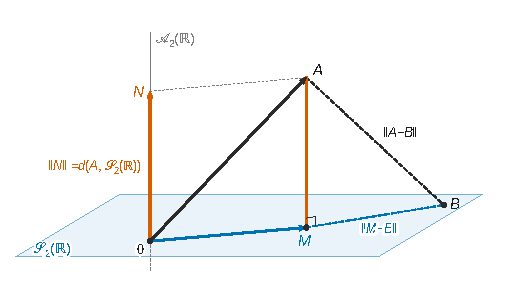
\includegraphics{figures/q24-projection-orthogonale.pdf}
\caption*{Figure 2 --- M est le projeté orthogonal de A sur 𝒮₂(ℝ) : pour toute B
symétrique, le triangle AMB est rectangle en M, donc d(A, 𝒮₂(ℝ)) = ‖N‖}
\end{figure}

\hypertarget{partie-ii-matrice-de-rademacher}{%
\section{Partie II --- Matrice de Rademacher}\label{partie-ii-matrice-de-rademacher}}

\hypertarget{q25}{%
\subsection{Q25}\label{q25}}

Par définition de l'espérance d'une variable finie :

\equationajustee{E(X_1)=(-1)\cdot\frac12+1\cdot\frac12=0.}

Comme \(X_1^2=1\), \(E(X_1^2)=1\). Par la formule de König-Huygens, \(V(X_1)=E(X_1^2)-E(X_1)^2=1\) :

\equationajustee{\boxed{\begin{aligned}E(X_1)&=0\\ V(X_1)&=1\end{aligned}}}

\hypertarget{q26}{%
\subsection{Q26}\label{q26}}

On a \(T_1(\Omega)=\{-2,0,2\}\). Par indépendance de \(X_1\) et \(Y_1\) :

\equationajustee{\begin{aligned}P(T_1=-2)&=P(X_1=-1)P(Y_1=-1)=\tfrac14\\ P(T_1=2)&=P(X_1=1)P(Y_1=1)=\tfrac14\end{aligned}}

L'événement \([T_1=0]\) est la réunion disjointe de \([X_1=-1]\cap[Y_1=1]\) et \([X_1=1]\cap[Y_1=-1]\). Par additivité et indépendance, \(P(T_1=0)=\frac14+\frac14=\frac12\).

\equationajustee{\boxed{\begin{aligned}P(T_1=-2)&=\tfrac14\\ P(T_1=0)&=\tfrac12\\ P(T_1=2)&=\tfrac14\end{aligned}}}

Espérance et moment d'ordre 2 :

\equationajustee{\begin{aligned}E(T_1)&=-2\cdot\tfrac14+0\cdot\tfrac12+2\cdot\tfrac14=0\\ E(T_1^2)&=4\cdot\tfrac14+0\cdot\tfrac12+4\cdot\tfrac14=2\end{aligned}}

Par König-Huygens, \(V(T_1)=E(T_1^2)-E(T_1)^2=2\) :

\equationajustee{\boxed{\begin{aligned}E(T_1)&=0\\ V(T_1)&=2\end{aligned}}}

(Contrôle : \(V(X_1)+V(Y_1)=2\) par indépendance.)

\hypertarget{q27}{%
\subsection{Q27}\label{q27}}

On a \(Z_1(\Omega)=\{-1,1\}\). L'événement \([Z_1=1]\) est la réunion disjointe de \([X_1=1]\cap[Y_1=1]\) et \([X_1=-1]\cap[Y_1=-1]\). Par indépendance, \(P(Z_1=1)=\frac14+\frac14=\frac12\), puis \(P(Z_1=-1)=\frac12\).

\textbf{\(Z_1\) suit la loi de Rademacher.} On a donc, comme en Q25 (avec \(Z_1^2=1\)) :

\equationajustee{\boxed{\begin{aligned}E(Z_1)&=0\\ V(Z_1)&=1\end{aligned}}}

\hypertarget{partie-iii-matrice-guxe9omuxe9trique}{%
\section{Partie III --- Matrice géométrique}\label{partie-iii-matrice-guxe9omuxe9trique}}

\hypertarget{q28}{%
\subsection{Q28}\label{q28}}

\equationajustee{\boxed{\begin{aligned}E(X_2)&=\frac1p\\ V(X_2)&=\frac{1-p}{p^2}\end{aligned}}}

\hypertarget{q29}{%
\subsection{Q29}\label{q29}}

\textbf{a)} Pour tout \(\omega\in\Omega\), on applique Q24 à la matrice \(A=\Sigma_2(\omega)\) :

\equationajustee{\begin{aligned}\Sigma_2-\Sigma_2^\top&=\begin{pmatrix}0&(X_2-Y_2)-(X_2+Y_2)\\(X_2+Y_2)-(X_2-Y_2)&0\end{pmatrix}\\ &=\begin{pmatrix}0&-2Y_2\\2Y_2&0\end{pmatrix}.\end{aligned}}

Par Q20, \(\|\Sigma_2-\Sigma_2^\top\|^2=8Y_2^2\), donc \(\|\Sigma_2-\Sigma_2^\top\|=2\sqrt2\,|Y_2|=2\sqrt2\,Y_2\), car \(Y_2\ge1>0\). Ainsi

\equationajustee{\boxed{T_2=\frac12\cdot2\sqrt2\,Y_2=\sqrt2\,Y_2.}}

\textbf{b)} \(Y_2\) suit la même loi géométrique que \(X_2\). Par linéarité de l'espérance et \(V(cY)=c^2V(Y)\) :

\equationajustee{\boxed{\begin{aligned}E(T_2)&=\frac{\sqrt2}p\\ V(T_2)&=\frac{2(1-p)}{p^2}\end{aligned}}}

\hypertarget{q30}{%
\subsection{Q30}\label{q30}}

\(T_2\) admet une variance (Q29 b). L'inégalité de Bienaymé-Tchebychev donne, pour tout \(\delta>0\) :

\equationajustee{\boxed{\begin{aligned}P\Big(\Big|T_2-\frac{\sqrt2}p\Big|\ge\delta\Big)&\le\frac{V(T_2)}{\delta^2}\\ &=\frac{2(1-p)}{\delta^2p^2}.\end{aligned}}}

\hypertarget{q31}{%
\subsection{Q31}\label{q31}}

\textbf{a)} Pour \(p=\frac12\) : \(\frac{\sqrt2}p=2\sqrt2\) et \(\frac{2(1-p)}{\delta^2p^2}=\frac4{\delta^2}\). Or, pour \(\delta>0\) :

\equationajustee{\frac4{\delta^2}\le\frac14\iff\delta\ge4.}

\textbf{Pour \(\delta=4\)} :

\equationajustee{\boxed{P\big(|T_2-2\sqrt2|\ge4\big)\le\frac14.}}

\textbf{b)} En passant à l'événement contraire :

\equationajustee{P\big(|T_2-2\sqrt2|<4\big)\ge1-\frac14=\frac34.}

Comme \(T_2=d(\Sigma_2,\mathcal S_2(\mathbb R))\) :

\equationajustee{\boxed{P\Big(\big|d(\Sigma_2,\mathcal S_2(\mathbb R))-2\sqrt2\big|<4\Big)\ge\frac34.}}

\begin{figure}[H]
\centering
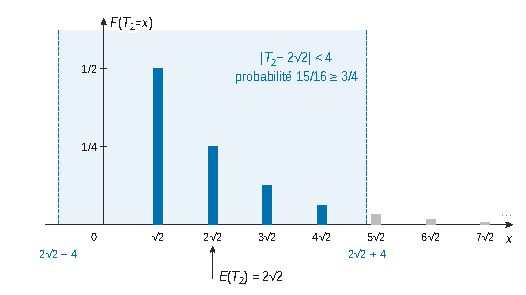
\includegraphics{figures/q31-loi-t2-tchebychev.pdf}
\caption*{Figure 3 --- Loi de T₂ pour p = 1/2 : l'intervalle \textbar T₂ −
2√2\textbar{} \textless{} 4 contient k = 1 à 4, de probabilité 15/16 au
lieu du 3/4 garanti}
\end{figure}

\hypertarget{partie-iv-matrice-de-poisson}{%
\section{Partie IV --- Matrice de Poisson}\label{partie-iv-matrice-de-poisson}}

\hypertarget{q32}{%
\subsection{Q32}\label{q32}}

\equationajustee{\boxed{\begin{aligned}E(X_3)&=\lambda\\ V(X_3)&=\lambda\end{aligned}}}

\hypertarget{q33}{%
\subsection{Q33}\label{q33}}

\textbf{a)} Un produit de réels est nul si et seulement si l'un des facteurs l'est : \([Z_3=0]=[X_3=0]\cup[Y_3=0]\). Par la formule de la probabilité de la réunion de deux événements, \(P(A\cup B)=P(A)+P(B)-P(A\cap B)\), puis par indépendance de \(X_3\) et \(Y_3\) :

\equationajustee{\begin{aligned}P(Z_3=0)&=P(X_3=0)+P(Y_3=0)-P(X_3=0)P(Y_3=0)\\ &=e^{-\lambda}+e^{-\lambda}-e^{-\lambda}e^{-\lambda}\end{aligned}}

\equationajustee{\boxed{P(Z_3=0)=2\exp(-\lambda)-\exp(-2\lambda).}}

\textbf{b)} On a \(\det\Sigma_3=X_3Y_3=Z_3\), et \(\Sigma_3\) est inversible si et seulement si \(Z_3\ne0\). Par passage au contraire :

\equationajustee{\boxed{\begin{aligned}P(\Sigma_3\ \text{inversible})&=1-2e^{-\lambda}+e^{-2\lambda}\\ &=\big(1-e^{-\lambda}\big)^2.\end{aligned}}}

\hypertarget{q34}{%
\subsection{Q34}\label{q34}}

\textbf{a)} \emph{Support.} \(X_3\) et \(Y_3\) sont à valeurs dans \(\mathbb N\), donc \(T_3(\Omega)\subset\mathbb N\). Réciproquement, soit \(n\in\mathbb N\) ; par indépendance,

\equationajustee{\begin{aligned}P\big([X_3=n]\cap[Y_3=0]\big)&=e^{-2\lambda}\frac{\lambda^n}{n!}\\ &>0.\end{aligned}}

Cet événement est donc non vide, et sur lui \(T_3=n\) : \(n\in T_3(\Omega)\). \textbf{Donc \(T_3(\Omega)=\mathbb N\).}

\emph{Formule.} La famille \(([X_3=k])_{k\in\mathbb N}\) est un système complet d'événements. Par la formule des probabilités totales :

\equationajustee{\begin{aligned}P(T_3=n)&=\sum_{k=0}^{+\infty}P\big([X_3=k]\cap[T_3=n]\big)\\ &=\sum_{k=0}^{+\infty}P\big([X_3=k]\cap[Y_3=n-k]\big).\end{aligned}}

Pour \(k>n\), l'événement \([Y_3=n-k]\) est vide, car \(Y_3\ge0\) : ces termes sont nuls. Par indépendance de \(X_3\) et \(Y_3\) :

\equationajustee{\boxed{\begin{aligned}{}&\forall n\in\mathbb N,\\ &P(T_3=n)=\sum_{k=0}^nP(X_3=k)\,P(Y_3=n-k).\end{aligned}}}

\textbf{b)} Soit \(n\in\mathbb N\). En reportant les lois de Poisson :

\equationajustee{\begin{aligned}P(T_3=n)&=\sum_{k=0}^ne^{-\lambda}\frac{\lambda^k}{k!}\,e^{-\lambda}\frac{\lambda^{n-k}}{(n-k)!}\\ &=e^{-2\lambda}\frac{\lambda^n}{n!}\sum_{k=0}^n\binom nk\\ &=e^{-2\lambda}\frac{(2\lambda)^n}{n!},\end{aligned}}

par la formule du binôme (\(\sum_{k=0}^n\binom nk=2^n\)). \textbf{\(T_3\) suit la loi de Poisson de paramètre \(2\lambda\).}

\hypertarget{q35}{%
\subsection{Q35}\label{q35}}

\textbf{a)} Le vecteur \(V=\begin{pmatrix}X_3-Y_3\\1\end{pmatrix}\) est non nul, car sa seconde coordonnée vaut \(1\). On calcule :

\equationajustee{\begin{aligned}\Sigma_3V&=\begin{pmatrix}X_3(X_3-Y_3)\\X_3-Y_3+Y_3\end{pmatrix}\\ &=X_3\begin{pmatrix}X_3-Y_3\\1\end{pmatrix}.\end{aligned}}

\textbf{\(V\) est vecteur propre de \(\Sigma_3\) associé à la valeur propre \(X_3\).}

\textbf{b)} Le vecteur \(W=\begin{pmatrix}0\\1\end{pmatrix}\) est non nul, et \(\Sigma_3W=\begin{pmatrix}0\\Y_3\end{pmatrix}=Y_3W\). \textbf{\(Y_3\) est valeur propre de \(\Sigma_3\), de vecteur propre associé \(\begin{pmatrix}0\\1\end{pmatrix}\).}

\hypertarget{q36}{%
\subsection{Q36}\label{q36}}

\textbf{a)} La famille \(([Y_3=k])_{k\in\mathbb N}\) est un système complet d'événements. Par la formule des probabilités totales :

\equationajustee{\begin{aligned}P(X_3=Y_3)&=\sum_{k=0}^{+\infty}P\big([X_3=Y_3]\cap[Y_3=k]\big)\\ &=\sum_{k=0}^{+\infty}P\big([X_3=k]\cap[Y_3=k]\big).\end{aligned}}

Par indépendance de \(X_3\) et \(Y_3\), puis égalité de leurs lois :

\equationajustee{\boxed{\begin{aligned}P(X_3=Y_3)&=\sum_{k=0}^{+\infty}P(X_3=k)P(Y_3=k)\\ &=\sum_{k=0}^{+\infty}P(X_3=k)^2.\end{aligned}}}

\textbf{b)} Fixons \(\omega\) et posons \(x=X_3(\omega)\), \(y=Y_3(\omega)\).

\begin{itemize}
\tightlist
\item
  \emph{Si \(x\ne y\)} : par Q35, \(\Sigma_3\), d'ordre 2, a deux valeurs propres réelles distinctes \(x\) et \(y\), donc est diagonalisable dans \(\mathbb R\).
\item
  \emph{Si \(x=y=c\)} : \(\Sigma_3=\begin{pmatrix}c&0\\1&c\end{pmatrix}\) est triangulaire, de seule valeur propre \(c\). Si elle était diagonalisable, elle serait semblable à \(cI_2\), donc égale à \(P(cI_2)P^{-1}=cI_2\).
  Or son coefficient \((2,1)\) vaut \(1\) : contradiction.
\end{itemize}

On a montré les deux implications :

\equationajustee{\boxed{\Sigma_3\ \text{est diagonalisable dans}\ \mathbb R\iff X_3\ne Y_3.}}

\textbf{c)} Par b), \(D_\lambda=[X_3\ne Y_3]\). Par a), en passant au contraire :

\equationajustee{P(D_\lambda)=1-\sum_{k=0}^{+\infty}\Big(e^{-\lambda}\frac{\lambda^k}{k!}\Big)^2,}

\equationajustee{\boxed{P(D_\lambda)=1-e^{-2\lambda}\sum_{k=0}^{+\infty}\frac{\lambda^{2k}}{(k!)^2}.}}

\hypertarget{q37}{%
\subsection{Q37}\label{q37}}

\textbf{a)}

\begin{lstlisting}[language=Python]
import math

def Approx_Sum(N):
    S = 0
    for k in range(N + 1):          # k = 0, 1, ..., N
        S = S + math.exp(-2) / math.factorial(k) ** 2
    return S
\end{lstlisting}

(Exécution : \texttt{Approx\_Sum(4)} renvoie \(0{,}30850\ldots\))

\textbf{b)} \emph{Formule de Taylor avec reste intégral} : si \(\varphi\) est de classe \(\mathcal C^{n+1}\) sur un intervalle \(I\) et \(a,x\in I\), alors

\equationajustee{\varphi(x)=\sum_{k=0}^n\frac{\varphi^{(k)}(a)}{k!}(x-a)^k+\int_a^x\frac{(x-t)^n}{n!}\varphi^{(n+1)}(t)\,\mathrm dt.}

On l'applique à \(\varphi=\exp\), qui est de classe \(\mathcal C^\infty\), donc \(\mathcal C^{n+1}\), sur \(I=\mathbb R\). On prend \(a=0\) et \(x\ge0\).

Toutes les dérivées de \(\exp\) valent \(\exp\), et \(\exp(0)=1\) :

\equationajustee{\boxed{\begin{aligned}{}&\forall n\in\mathbb N,\ \forall x\ge0,\\ &\exp(x)-\sum_{k=0}^n\frac{x^k}{k!}=\frac1{n!}\int_0^x(x-t)^n\exp(t)\,\mathrm dt.\end{aligned}}}

\textbf{c)} Soit \(x\ge0\). Pour \(t\in[0,x]\), \(\exp\) étant croissante :

\equationajustee{0\le(x-t)^ne^t\le(x-t)^ne^x.}

Par croissance de l'intégrale (bornes \(0\le x\)), avec \(\int_0^x(x-t)^n\,\mathrm dt=\frac{x^{n+1}}{n+1}\) :

\equationajustee{\begin{aligned}0\le\exp(x)-\sum_{k=0}^n\frac{x^k}{k!}&\le\frac{e^x}{n!}\cdot\frac{x^{n+1}}{n+1}\\ &=\frac{x^{n+1}}{(n+1)!}\exp(x).\end{aligned}}

\equationajustee{\boxed{\exp(x)-\sum_{k=0}^n\frac{x^k}{k!}\le\frac{x^{n+1}}{(n+1)!}\exp(x).}}

\textbf{d)} Avec \(x=1\) dans c), pour tout \(n\) :

\equationajustee{\begin{aligned}0&\le e-\sum_{k=0}^n\frac1{k!}\\ &\le\frac e{(n+1)!}.\end{aligned}}

Le majorant tend vers \(0\) quand \(n\to+\infty\). Donc \(\sum_{k\ge0}\frac1{k!}\) converge et vaut \(e\), et son reste vérifie :

\equationajustee{\boxed{\begin{aligned}\sum_{k=n+1}^{+\infty}\frac1{k!}&=e-\sum_{k=0}^n\frac1{k!}\\ &\le\frac e{(n+1)!}.\end{aligned}}}

\textbf{e)} Pour \(k\in\mathbb N\), \(k!\ge1\), donc \(0\le\frac1{(k!)^2}\le\frac1{k!}\). La série \(\sum\frac{e^{-2}}{(k!)^2}\), à termes positifs, converge par comparaison. Son reste d'ordre \(n\) est positif, et par d) :

\equationajustee{\begin{aligned}\sum_{k=0}^{+\infty}\frac{e^{-2}}{(k!)^2}-\sum_{k=0}^n\frac{e^{-2}}{(k!)^2}&=\sum_{k=n+1}^{+\infty}\frac{e^{-2}}{(k!)^2}\\ &\le e^{-2}\sum_{k=n+1}^{+\infty}\frac1{k!}\\ &\le e^{-2}\frac e{(n+1)!}=\frac{e^{-1}}{(n+1)!}.\end{aligned}}

\equationajustee{\boxed{\begin{aligned}0&\le\sum_{k=0}^{+\infty}\frac{e^{-2}}{(k!)^2}-\sum_{k=0}^n\frac{e^{-2}}{(k!)^2}\\ &\le\frac{e^{-1}}{(n+1)!}.\end{aligned}}}

\textbf{f)} Par e), il suffit que \(\frac{e^{-1}}{(N_0+1)!}\le10^{-2}\), c'est-à-dire \((N_0+1)!\ge100e^{-1}\). Comme \(100e^{-1}\le37\), il suffit que \((N_0+1)!\ge37\).

Or \(4!=24<37\) mais \(5!=120\ge37\). \textbf{\(N_0=4\) convient} :

\equationajustee{\begin{aligned}\Big|\sum_{k=0}^{+\infty}\frac{e^{-2}}{(k!)^2}-\sum_{k=0}^{4}\frac{e^{-2}}{(k!)^2}\Big|&\le\frac{e^{-1}}{120}\\ &\le\frac{0{,}37}{120}<10^{-2}.\end{aligned}}

(Avec cette majoration, \(N_0=3\) ne suffit pas : \(4!=24<36\le100e^{-1}\).)

\textbf{g)} Notons \(S=\sum_{k\ge0}\frac{e^{-2}}{(k!)^2}\). La valeur affichée \(0{,}31\) est un arrondi au centième : \(\texttt{Approx\_Sum}(4)\in[0{,}305\,;0{,}315[\).

Par e) et f), \(0\le S-\texttt{Approx\_Sum}(4)\le10^{-2}\), donc \(S\in[0{,}305\,;0{,}325]\) :

\equationajustee{\boxed{S\approx0{,}3\ \text{\text{à}}\ 10^{-1}\ \text{\text{près}}.}}

Par Q36 c) avec \(\lambda=1\), \(P(D_1)=1-e^{-2}\sum_{k\ge0}\frac1{(k!)^2}=1-S\), donc \(P(D_1)\in[0{,}675\,;0{,}695]\) :

\equationajustee{\boxed{P(D_1)\approx0{,}7\ \text{\text{à}}\ 10^{-1}\ \text{\text{près}}.}}

(Valeurs plus précises : \(S\approx0{,}3085\) et \(P(D_1)\approx0{,}6915\).)

\textbf{h)} Ce n'est pas judicieux en général. L'appel \texttt{math.factorial(\allowbreak{}k)\allowbreak{}} recalcule \(k!\) à partir de zéro, soit environ \(k\) multiplications à chaque tour.

Au total, cela fait de l'ordre de \(\sum_{k=0}^Nk=\frac{N(N+1)}2\) multiplications (coût quadratique). En mettant à jour une variable par \(k!=(k-1)!\times k\), on n'en fait que \(N\) (coût linéaire) :

\begin{lstlisting}[language=Python]
def Approx_Sum_bis(N):
    S, f = 0, 1                     # f vaut k! au début du tour k
    for k in range(N + 1):
        if k > 0:
            f = f * k
        S = S + math.exp(-2) / f ** 2
    return S
\end{lstlisting}

Ici \(N_0=4\) : la boucle fait 5 tours sur des entiers minuscules (\(0!,\dots,4!\)), soit une dizaine de multiplications au lieu de quatre. \textbf{Le surcoût est négligeable.}

\hypertarget{q38}{%
\subsection{Q38}\label{q38}}

\textbf{a)} Soit \(x\ne0\) et \(u_k=\frac{x^k}{(k!)^2}\ne0\). On a

\equationajustee{\left|\frac{u_{k+1}}{u_k}\right|=\frac{|x|}{(k+1)^2}\xrightarrow[k\to+\infty]{}0<1.}

Par la règle de d'Alembert, la série converge absolument pour tout réel \(x\) :

\equationajustee{\boxed{R=+\infty.}}

\textbf{b)} La somme d'une série entière est continue sur son intervalle ouvert de convergence, ici \(]-\infty,+\infty[\). \textbf{Donc \(h:x\mapsto\sum_{k\ge0}\frac{x^k}{(k!)^2}\) est continue sur \(\mathbb R\).}

\textbf{c)} Pour \(\lambda\ge0\), on a \(g(\lambda)=1-e^{-2\lambda}h(\lambda^2)\).

Les fonctions \(\lambda\mapsto\lambda^2\), \(h\) (b) et \(\lambda\mapsto e^{-2\lambda}\) sont continues. Par composition, produit et somme, \textbf{\(g\) est continue sur \([0,+\infty[\).}

\hypertarget{q39}{%
\subsection{Q39}\label{q39}}

Soit \(\lambda>0\), et \(X_3,Y_3\) indépendantes de loi \(\mathcal P(\lambda)\).

Par Q36 c), la probabilité que \(\begin{pmatrix}X_3&0\\1&Y_3\end{pmatrix}\) soit diagonalisable est \(P(D_\lambda)=g(\lambda)\). Il suffit donc de trouver \(\mu>0\) tel que \(g(\mu)=\frac12\).

\begin{itemize}
\tightlist
\item
  \(g(0)=1-e^0\cdot1=0\) (seul le terme \(k=0\) de la série est non nul).
\item
  Comme \(\frac1{(k!)^2}\le\frac1{k!}\), on a \(\sum_{k\ge0}\frac1{(k!)^2}\le e\) (Q37 d). Donc :
\end{itemize}

\equationajustee{\begin{aligned}g(1)&\ge1-e^{-2}e=1-e^{-1}\\ &\ge1-0{,}37=0{,}63>\tfrac12.\end{aligned}}

\(g\) est continue sur \([0,1]\) (Q38 c), avec \(g(0)<\frac12<g(1)\).

Par le théorème des valeurs intermédiaires, il existe \(\mu\in[0,1]\) tel que \(g(\mu)=\frac12\), et \(\mu\ne0\) car \(g(0)=0\).

\equationajustee{\boxed{\begin{aligned}{}&\exists\,\mu\in\,]0,1[,\ \text{pour}\ X_3,Y_3\sim\mathcal P(\mu)\ \text{\text{indépendantes}}:\\ &P\left(\begin{pmatrix}X_3&0\\1&Y_3\end{pmatrix}\ \text{diagonalisable}\right)=g(\mu)=\frac12.\end{aligned}}}

\begin{figure}[H]
\centering
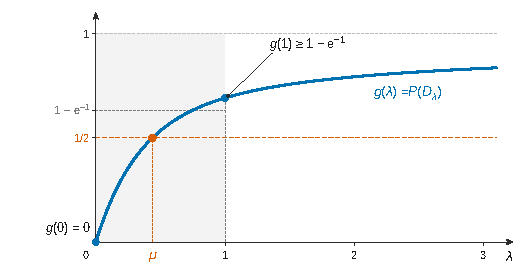
\includegraphics{figures/q39-graphe-g-valeurs-intermediaires.pdf}
\caption*{Figure 4 --- Graphe de g : g(0) = 0 et g(1) ≥ 1 − e⁻¹ \textgreater{}
1/2, donc g prend la valeur 1/2 en un μ compris entre 0 et 1}
\end{figure}

\hypertarget{q40}{%
\subsection{Q40}\label{q40}}

On applique la \textbf{méthode de dichotomie} à \(\varphi=g-\frac12\), continue sur \([0,1]\), avec \(\varphi(0)<0<\varphi(1)\) (Q39) :

\begin{enumerate}
\def\labelenumi{\arabic{enumi}.}
\tightlist
\item
  \(u\leftarrow0\), \(v\leftarrow1\) ;
\item
  tant que \(v-u>\varepsilon\) : \(m\leftarrow\frac{u+v}2\) ; si \(\varphi(m)<0\), \(u\leftarrow m\), sinon \(v\leftarrow m\) ;
\item
  renvoyer \(\frac{u+v}2\).
\end{enumerate}

L'invariant \(\varphi(u)<0\le\varphi(v)\) et le théorème des valeurs intermédiaires assurent qu'un zéro de \(\varphi\) reste dans \([u,v]\). La longueur de cet intervalle est divisée par 2 à chaque étape : \(\lceil\log_2(1/\varepsilon)\rceil\) itérations suffisent (une dizaine pour \(\varepsilon=10^{-3}\)).

Chaque évaluation de \(g(m)\) se fait en tronquant la série :

\equationajustee{g(m)\simeq1-e^{-2m}\sum_{k=0}^K\frac{m^{2k}}{(k!)^2}.}

Pour \(m\in[0,1]\), l'erreur est majorée par \(\sum_{k>K}\frac1{k!}\le\frac e{(K+1)!}\) (comme en Q37 d--e). \(K=8\) donne une erreur \(<10^{-5}\), et la factorielle est mise à jour par une multiplication (Q37 h). On obtiendrait \(\mu\approx0{,}44\).

\textbf{FIN}

\end{document}
